 % ewic.tex for classfile V2.04, 6 July 2011

\documentclass{ewic}
%\documentclass[cm]{ewic}
\usepackage{graphicx,wrapfig,subfig}
\begin{document}

\runningheads{Ferrari $\bullet$ Mazzanti $\bullet$ Spagnolo}{A model checker solution for the deadlock free the subway}

\conference{Proceedings of  International Workshop on Verification and Evaluation of Computer and Communication Systems 2013}

\title{A model checker solution for the deadlock free the subway[tp]}

\authorone{Alessio Ferrari\\
ISTI-CNR\\
via G. Moruzzi 1 \\56124 Pisa\\
 ITALY\\
fmt.isti.cnr.it\\
\email{alessio.ferrari@isti.cnr.it}}

\authortwo{Franco Mazzanti\\
ISTI-CNR\\
via G. Moruzzi 1\\
56124 Pisa \\
ITALY\\
fmt.isti.cnr.it\\
\email{franco.mazzanti@isti.cnr.it}}

\authorthree{Giorgio O. Spagnolo\\
ISTI-CNR\\
via G. Moruzzi 1 \\
56124 Pisa\\
 ITALY\\
fmt.isti.cnr.it\\
\email{spagnolo@isti.cnr.it}}


\begin{abstract}
This is an abstract.
\end{abstract}

\keywords{Automatic Train Supervisor, CBTC, Deadlock, UMC, Railway, Subway}

\maketitle

\section{Introduction}

This paper describes the ewic.cls class file which can be used to
convert articles produced with other \LaTeXe\ class files into the
correct form for publication by \emph{Electronic Workshops in
Computing}.

The ewic.cls class file preserves much of the standard \LaTeXe\
interface so that any document which has been produced using the
standard \LaTeXe\ article style can easily be converted to work
with the ewic style. However, the width of text and typesize may
vary from that of \emph{article}; therefore \emph{line breaks will
change} and it is possible that computer listings and displayed
mathematics may need resetting.

In the following sections we describe how to lay out your code to
use ewic.cls to reproduce the typographical look required for
online publication. However, this short paper is not a guide to
using \LaTeXe\ and we would refer you to any of the many books
available (see, for example, \cite{Companion,KopkaDaly,Lamport}).

\subsection{eWiC: Information for Authors}
You should also consult \emph{eWiC: Information for Authors} (available
from the BCS website) for important instructions about submission,
style and preparation of your paper.
[studio preliminare]


\section{Background}
%\input{back}
\begin{enumerate}
\item Contesto ferroviario: Metropolitate CBTC
\item Il sistema CBTC
\item L'ATS il suo compito -> Routing vs TimeTable
\item definizione di tabella orario
\item definizione di missione
\item sicurezza dei treni divisione della linea in blocchi
\item definizione di itinerario 
\item definizione di deadlock in sistema ferroviario
\end{enumerate}



\section{Pattern Deadlock definition}
\begin{itemize}
\item definizione della rappresentazione usata
\item definizione dei deadlock di base:
\item dritto, cicolare o composizione dei precedenti
\end{itemize}

\section{Method overview}


%Dati il layout di una metropolitana e la tabella orario dei treni che si vogliono far circolare. Viene definito il modello delle missioni dei singoli treni. Il modello delle missioni unito al modello dello stato della linea formano il modello di scheduling del sistema. 
%Il risultato dell'analisi del model chec ker 

%In questo paragrafo noi descriviamo l'approccio utilizzato per verificare ed eliminare i deadlock in una metropolitana.
%In particolare questa è l'analisi fatta dall'ATS per schedulare i treni in caso di ritardo senza generare deadlock.

In this section we describe the approach used to verify and delete deadlock in a subway.
In particular, this is the analysis performed by the ATS to schedule trains in case of delay without generating deadlocks.

%Il nostro approccio si basa sull'utilizzo iterativo di un model checker per verificare la presenza di deadlock di una metropolitana.

Our approach is based on an iterative model checker to verify the presence of deadlocks of a subway.

\begin{figure}[h!]
	\begin{centering}	
	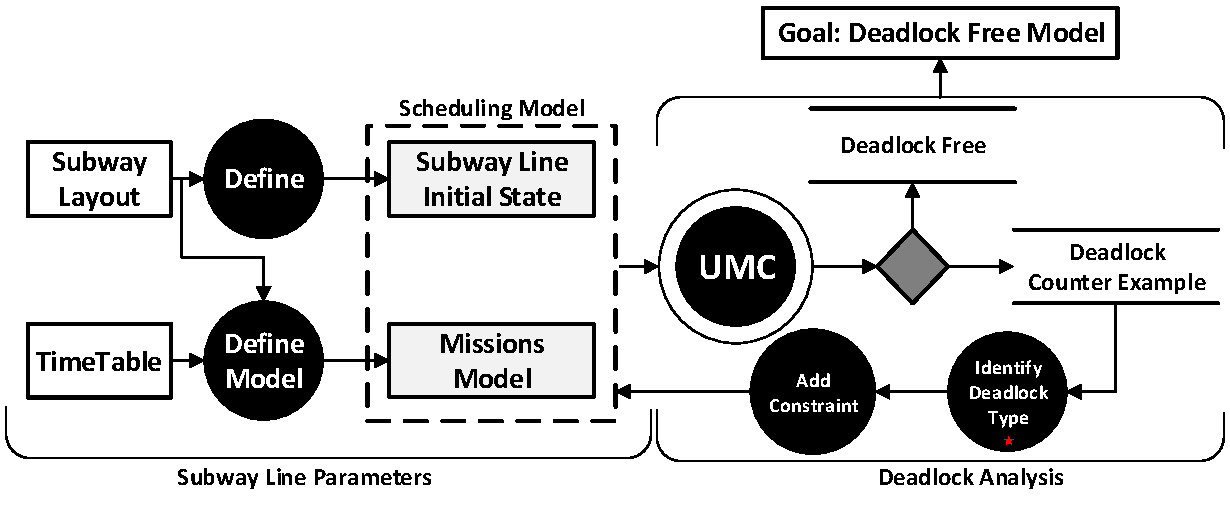
\includegraphics[width=0.45\textwidth, clip]{img/processo}
	\caption{Overview of the approach}
	\label{fig:process}
	\end{centering}
\end{figure}

%La figura~\ref{fig:process} descrive graficamente l'approccio usato.
The figure ~\ref{fig:process} describes the approach used.

%%Nella prima fase, che chiamiamo SLP, vengo preparati i dati per effettuare l'analisi di deadlock della linea.
%I dati di partenza sono  il layout della metropolitana e la tabella orario dei treni che si vogliono far circolare. Questi dati sono usati per definire i modelli delle missioni dei singoli treni. 

The source data are the subway  layout and the metro timetable. Both are used to define models of the missions of individual trains, see figure~\ref{fig:lmissionm}.


%Invece il layout della metropolitana viene usato anche per definire lo stato iniziale della linea. Cosi è possibile bloccare alcuni tratti di metropolitana perchè impegnati ad esempio da lavori di manutenzione.

Whereas the layout of the subway is also used to define the initial state of the line, see figure~\ref{fig:lstateline}. So you can lock some parts of the subway because it involved such as maintenance or insert the initial position of train.

%I modelli di missione e lo stato iniziale della metropolitana costituiscono il modello di scheduling della metropolitana.

The models of the mission and the model initial state of the subway they represent the model of scheduling of the subway, see figure~\ref{fig:SchedulingModel}.

%Il modello di scheduling viene analizzato tramite il model checker UMC[inserire riferimento]
The scheduling model is analyzed using the model checker UMC [insert reference]
%UMC permette di specificare come un insime di statecharts UML e di verificare proprità relative all'evoluzione del sistema. 
UMC allows to specify a system as a set of UML Statecharts and verify properties related to the evolution of the system.

%Se risultato del modelchecker è controesempio di deadlock. Si identificano i pattern di deadlock e si inserisco delle nuove regole nelle aree scritiche identificate. Altrimenti potremo affermare che il modello è libero di deadlock.

If the result of the model checker is deadlock counter example we identify patterns of deadlocks and insert the new contraints in the critical areas identified, see section~\ref{sec:deadlockpatterndefinition}. Otherwise, we can conclude that the model is free of deadlocks. 
%Quindi tutti i treni sono ingrado di arrivare a destinazione senza generare deadlock.
So all the trains, present into timetable, are able to arrive at your destination without generating deadlock.

\section{DeadLock Analysis}
\begin{enumerate}
\item introduzione del caso concreto
\item presentazione layout dell'esempio
\item presentazione di una sez di tab orario
\item \ldots
\end{enumerate}
%\input{example}

\section{Related works}
%\input{releted}
\section{Conclusion}
%\input{conclusion}



\pagebreak
\subsection{Notes}
\begin{enumerate}
\item Please separate multiple author surnames by a `\verb+$\bullet$+' within the
\verb+\runningheads{}{}+ command.

\item The class file is set up to handle up to six authors, i.e., \verb+\authorone{}...\authorsix{}+.

\item Note that the required reference style is Harvard. ewic.cls
uses `natbib.sty' to achieve the desired output so you will need
to choose a natbib compatible .bst that gives Harvard style
output. `chicago.bst' would be a good choice.

\item Try to balance the columns on the final page when your paper is submitted.
\end{enumerate}

That really is all you should need to know to prepare your paper
using ewic.cls.\citep{Mills2003}

You do, of course, have the option to call in any of your
favourite packages for setting maths, graphics, computer listings,
etc.

\textbf{Acknowledgments. }
This work was partially supported by the PAR FAS 2007-2013 (TRACE-IT) project.

%\begin{thebibliography}{9}
%
%\bibitem[Kopka and Daly(2004)]{KopkaDaly}
%Kopka, H. and Daly, P.W.  (2004) \textit{A Guide to \LaTeXe:
%Document Preparation for Beginners and Advanced Users} (4th~edn).
%Addison-Wesley.
%
%\bibitem[Lamport(1994)]{Lamport}
%Lamport L. (1994) \textit{\LaTeX: A Document Preparation System}
%(2nd~edn). Addison-Wesley.
%
%\bibitem[Mittelbach and Goossens(2004)]{Companion}
%Mittelbach, F. and Goossens, M., (2004) \textit{The \LaTeX\
%Companion} (2nd~edn). Addison-Wesley.
%
%\end{thebibliography}

\bibliographystyle{chicago}
\bibliography{bibliography}


\end{document}
